\documentclass[border=12pt,tikz]{standalone}
\usepackage[T1]{fontenc}
\usepackage{lmodern}
\usepackage[dvipsnames]{xcolor}
\usetikzlibrary{arrows.meta,positioning,calc,fit,backgrounds}

\definecolor{ink}{HTML}{1A1A1A}
\definecolor{accent}{HTML}{2a78d6}
\definecolor{warn}{HTML}{eb6834}
\definecolor{band}{HTML}{F3F6F9}
\definecolor{accentbg}{HTML}{E9F0F7}
\definecolor{warnbg}{HTML}{FCEFE9}

\hyphenpenalty=10000 \exhyphenpenalty=10000 \tolerance=9999

\begin{document}
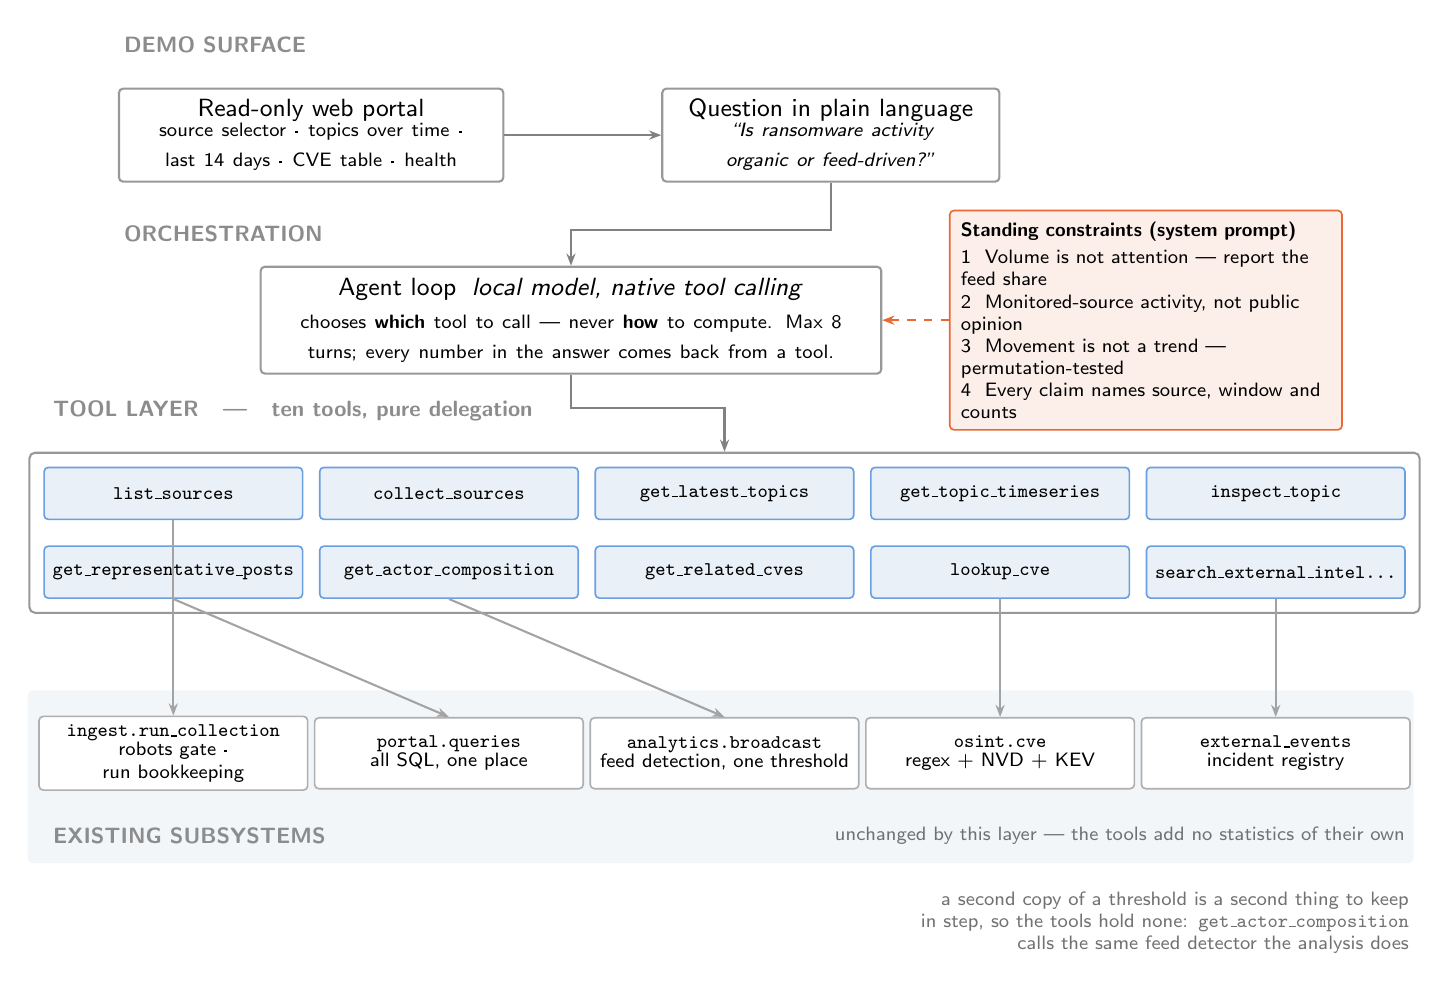
\begin{tikzpicture}[
  font=\sffamily\small, x=1cm, y=1cm,
  box/.style={draw=ink!45, fill=white, rounded corners=1.5pt, line width=.75pt,
              align=center, inner sep=4pt, text width=#1, minimum height=10mm},
  box/.default=40mm,
  tool/.style={draw=accent!70, fill=accentbg, rounded corners=1.5pt,
               line width=.6pt, align=center, font=\sffamily\scriptsize\ttfamily,
               inner sep=2.6pt, text width=31mm, minimum height=6.6mm},
  back/.style={draw=ink!35, fill=white, rounded corners=1.5pt, line width=.6pt,
               align=center, font=\sffamily\scriptsize, inner sep=3pt,
               text width=32mm, minimum height=9mm},
  rail/.style={draw=warn, fill=warnbg, rounded corners=1.5pt, line width=.6pt,
               align=left, font=\sffamily\scriptsize, inner sep=4pt,
               text width=47mm},
  hdr/.style={font=\sffamily\footnotesize\bfseries, text=ink!50},
  ann/.style={font=\sffamily\scriptsize, text=ink!62, align=center, inner sep=1.5pt},
  ar/.style={-{Stealth[length=4.4pt]}, draw=ink!55, line width=.75pt},
]

%% ================= row 1 : the demo surface =================
\node[box=46mm] (portal) at (0,0)
  {Read-only web portal\\[-1pt]{\scriptsize source selector · topics over time ·\\last 14 days · CVE table · health}};
\node[box=40mm] (ask) at (6.6,0)
  {Question in plain language\\[-1pt]{\scriptsize \textit{``Is ransomware activity\\organic or feed-driven?''}}};
\node[hdr, anchor=west] at (-2.5,1.15) {DEMO SURFACE};

\draw[ar] (portal) -- (ask);

%% ================= row 2 : the agent loop =================
\node[box=76mm] (loop) at (3.3,-2.35)
  {Agent loop \;\textit{local model, native tool calling}\\[1pt]
   {\scriptsize chooses \textbf{which} tool to call --- never \textbf{how} to compute.
   Max 8 turns; every number in the answer comes back from a tool.}};
\node[hdr, anchor=west] at (-2.5,-1.25) {ORCHESTRATION};

\node[rail, anchor=west] (guards) at (8.1,-2.35)
  {\textbf{Standing constraints (system prompt)}\\[2pt]
   1 \ Volume is not attention --- report the feed share\\
   2 \ Monitored-source activity, not public opinion\\
   3 \ Movement is not a trend --- permutation-tested\\
   4 \ Every claim names source, window and counts};

\draw[ar] (ask.south) -- ++(0,-.6) -| (loop.north);
\draw[ar, draw=warn, dashed] (guards.west) -- (loop.east);

%% ================= row 3 : the tool layer =================
\node[tool] (t1) at (-1.75,-4.55) {list\_sources};
\node[tool] (t2) at ( 1.75,-4.55) {collect\_sources};
\node[tool] (t3) at ( 5.25,-4.55) {get\_latest\_topics};
\node[tool] (t4) at ( 8.75,-4.55) {get\_topic\_timeseries};
\node[tool] (t5) at (12.25,-4.55) {inspect\_topic};
\node[tool] (t6) at (-1.75,-5.55) {get\_representative\_posts};
\node[tool] (t7) at ( 1.75,-5.55) {get\_actor\_composition};
\node[tool] (t8) at ( 5.25,-5.55) {get\_related\_cves};
\node[tool] (t9) at ( 8.75,-5.55) {lookup\_cve};
\node[tool] (ta) at (12.25,-5.55) {search\_external\_intel...};
\begin{scope}[on background layer]
  \node[draw=ink!45, fill=white, rounded corners=2pt, line width=.75pt,
        inner sep=5pt, fit=(t1)(t5)(t6)(ta)] (tools) {};
\end{scope}
\node[hdr, anchor=west] at (-3.4,-3.5) {TOOL LAYER \ \ --- \ \ ten tools, pure delegation};

\draw[ar] (loop.south) -- ++(0,-.42) -| (tools.north);

%% ================= row 4 : existing subsystems =================
\node[back] (b1) at (-1.75,-7.85) {\texttt{ingest.run\_collection}\\[-1pt]robots gate · run bookkeeping};
\node[back] (b2) at ( 1.75,-7.85) {\texttt{portal.queries}\\[-1pt]all SQL, one place};
\node[back] (b3) at ( 5.25,-7.85) {\texttt{analytics.broadcast}\\[-1pt]feed detection, one threshold};
\node[back] (b4) at ( 8.75,-7.85) {\texttt{osint.cve}\\[-1pt]regex $+$ NVD $+$ KEV};
\node[back] (b5) at (12.25,-7.85) {\texttt{external\_events}\\[-1pt]incident registry};
\begin{scope}[on background layer]
  \node[fill=band, rounded corners=2pt, inner sep=0pt,
        fit={(-3.6,-9.25) (14.0,-7.05)}] (backs) {};
\end{scope}
\node[hdr, anchor=west] at (-3.4,-8.9) {EXISTING SUBSYSTEMS};
\node[ann, anchor=east] at (13.95,-8.9)
  {unchanged by this layer --- the tools add no statistics of their own};

\foreach \a/\b in {t1/b1,t6/b2,t7/b3,t9/b4,ta/b5}
  \draw[ar, draw=ink!40] (\a.south) -- (\b.north);

\node[ann, anchor=north east, text width=62mm, align=right] at (14.0,-9.55)
  {a second copy of a threshold is a second thing to keep in step, so the
   tools hold none: \texttt{get\_actor\_composition} calls the same feed
   detector the analysis does};

\end{tikzpicture}
\end{document}
